
\documentclass[11pt]{report}
\usepackage{makeidx}
\usepackage{url}
\usepackage{a4wide}
\usepackage{longtable}
\usepackage{color}
\usepackage{alltt,xspace}
\usepackage{hyperref}
\usepackage{subfigure,graphicx,epsfig,epsf,amsmath,amsfonts,float}
\usepackage{fancyheadings}
\usepackage{relsize}
\usepackage{etoolbox} %% support for conditional compilation


\parskip5pt
\makeindex 
\parindent0pt
\sloppy 
\begin{document}
\newcommand{\FLORA}{{\mbox{\sc ${\cal F}${lora}\rm\emph{-2}}}\xspace}
\newcommand{\ERGO}{\ensuremath{\cal{E}\mbox{\smaller{\sc{RGO}}}}\xspace}
\newcommand{\ERGOLITE}{\ensuremath{\cal{E}\mbox{\smaller{\sc{RGO}\ensuremath{^{Lite}}}}}\xspace}
\newcommand{\FLSYSTEM}{\FLORA}
\newcommand{\FLRCFILE}{\texttt{FLORA\_RC\_FILE}\xspace}
\newcommand{\FLABORT}{FLORA\_ABORT}
\newcommand{\flabort}{'\_\$flora\_abort'}
\newcommand{\FLUSERABORT}{FLORA\_USER\_ABORT}
\newcommand{\FLUNDEFEXCEPTION}{FLORA\_UNDEFINED\_EXCEPTION}
\newcommand{\FLDBEXCEPTION}{FLORA\_DB\_EXCEPTION}
\newcommand{\flundefexception}{'\_\$flora\_undefined'}
\newcommand{\fldbexception}{'\_\$flora\_db\_error'}
\newcommand{\FLPREFIX}{\_\$\_\$\_flora}

\newcommand{\FLSHELL}{flora\_shell}
\newcommand{\FLBOOTSTRAP}{bootstrap\_flora}
\newcommand{\FLQUERYCMD}{flora\_query}

\newcommand{\ENGINENAME}{flora2}
\newcommand{\ENGINERUN}{runflora}

\newcommand{\prompt}{flora2 ?- }
\newcommand{\errorsystem}{Flora-2}
\newcommand{\flrext}{flr}

\IfFileExists{../ergoisms/ergo.switch}{\input{./ergoisms/definitions}}{\newcommand{\isfloraman}{yes}}

\newcommand{\fl}{F-logic }

\newcommand{\fd}{{\mbox{\tt \,->\,}}}                   % scalar
\newcommand{\mvd}{{\mbox{\tt \,->\,}}}  % multivalued
\newcommand{\Fd}{{\mbox{\tt \,=>\,}}}                      % scalar signature
\newcommand{\Mvd}{{\mbox{\tt \,=>\,}}}  % multivalued signature
\newcommand{\thismodule}{{\tt \_@}\xspace}
\newcommand{\bs}{{\ensuremath\backslash}}

\def\Protege{Prot\'{e}g\'{e} }
\def\NoProtege{Prot\'{e}g\'{e}}

\ifdef{\isfloraman}{
\title{\bf A Guide to \FLSYSTEM Packages
        \vspace{0.7cm}\\
 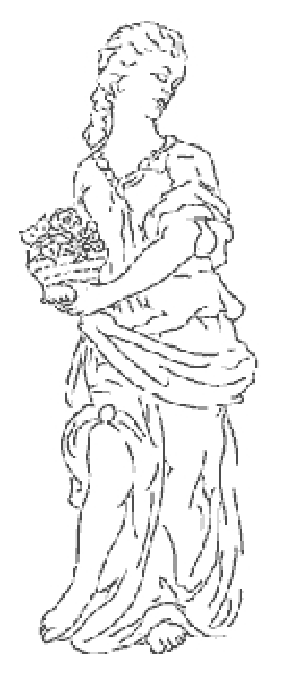
\includegraphics[width=1in]{floralogo} 
           \vspace{3mm}\\
       {\Large Version 1.1}
       \\
       {\large (Loquat)}
     }
     }
     {
       \input{./ergoisms/pkg-title}
     }


\date{}
\maketitle


\thispagestyle{empty}
\bibliographystyle{plain}
\newpage
\thispagestyle{empty}

\pagenumbering{roman}
\tableofcontents
\newpage        % Just to avoid a silly LaTeX bug with \pagenumbering
  
\pagenumbering{arabic}



\chapter[JAVA-to-\FLSYSTEM Interfaces]
{JAVA-to-\FLSYSTEM Interfaces\\
  {\Large by Aditi Pandit and Michael Kifer}}


This chapter documents the API for accessing \FLSYSTEM from Java
programs.  The API has two versions: a \emph{low-level API}, which
enables Java programs to send arbitrary queries to \FLSYSTEM and
get results, and a \emph{high-level API}, which is more limited,
but is easier to use. The high-level API establishes a
correspondence between Java classes and \FLSYSTEM classes, which
enables manipulation of \FLSYSTEM classes by executing appropriate
methods on the corresponding Java classes. Both interfaces rely on
the Java-XSB interface, called \emph{Interprolog}, developed by
\url{Interprolog.com}.

The API assumes that a Java program is started first and then it invokes
XSB/\FLSYSTEM as a subprocess. The XSB/\FLSYSTEM side is passive: it only
responds to the queries sent by the Java side.
Queries can be anything that is accepted at the \FLSYSTEM
shell prompt: queries, insert/delete commands, control switches, etc., are
all fine.
One thing to remember is that the backslash is used in Java
as an escape symbol and in \FLSYSTEM as a prefix of the builtin operators
and commands. Therefore, each backslash must be escaped with another
backslash. That is, instead of a query like "\texttt{p(?X) \bs{}and q(?X).}"
the API requires "\texttt{p(?X) \bs{}\bs{}and q(?X)}.".


\section{The Low-level Interface} \label{sec-java-lowlevel}
 The low-level API enables Java programs to send arbitrary queries
to \FLSYSTEM and get results. 
It is assumed that the following environment variables are set:

{\tt JAVA\_BIN}: This variable points to the folder containing
the javac and java executable programs. This variable is set in
the {\tt windowsVariables.bat} and  {\tt unixVariables.sh}  scripts in the
{\tt java} subfolder of the \FLSYSTEM distribution.

\texttt{PROLOGDIR}: 
This variable points to the folder
containing the XSB executable. This variable is set in the {\tt
  flora\_settings.bat} and {\tt flora\_settings.sh} scripts in the {\tt java}
folder. 

\label{page-floradir}
{\tt FLORADIR}: This variable must point to the folder
containing the \FLSYSTEM installation.
It is set by the {\tt
  flora\_settings.bat} and {\tt flora\_settings.sh} files in the {\tt java}
subfolder and this is where users should look in order to get the
correct values for their systems.
Both of the above files are generated automatically by the system installation
scripts.

In order to be able to access \FLSYSTEM, the Java program must first establish
a session for a running instance of \FLSYSTEM. Multiple sessions can be active
at the same time. The knowledge bases in the different running instances
are completely independent. Sessions are instances of
the class {\tt
javaAPI.src.FloraSession}. This class provides methods
for opening/closing sessions and loading \FLSYSTEM knowledge bases
(which are also used in the high-level
interface). In addition, a session provides 
methods for executing arbitrary \FLSYSTEM queries. The following is the complete
list of the methods that are available in that class.
%%
\begin{itemize}
\item
\begin{verbatim}
public FloraSession()
\end{verbatim}
  This method creates a connection to an instance of \FLSYSTEM.
\item {\tt close()} \\
  This method must be called to terminate a \FLSYSTEM session. Note that this does
  not terminate the Java program that initiated the session:
  to exit the Java program that talks to \FLSYSTEM, one needs to execute
  the statement
  %%
\begin{verbatim}
 System.exit();  
\end{verbatim}
  %%
  Note that just returning from the {\tt main} method is not enough. 

\item
\begin{verbatim}
public Iterator<FloraObject> ExecuteQuery(String command)
\end{verbatim}
    This method executes the \FLSYSTEM command given by the
parameter {\tt command}.  It is used to execute \FLSYSTEM queries that
do not require variable bindings to be returned back to Java or queries that
have only
a single variable to be returned. Each binding is represented as
an instance of the class {\tt javaAPI.src.FloraObject}.
The examples below illustrate how to process the results returned by this
method.

\item
\begin{verbatim}
public Iterator<HashMap<String,FloraObject>> ExecuteQuery(String query, Vector vars)
\end{verbatim}
  This method executes the \FLSYSTEM query given by the first argument. The
  Vector {\tt vars} (of strings) specifies the names of all the variables
  in the query for which bindings need to be returned. These variables are
  added to the vector using the method {\tt add} before calling
  {\tt ExecuteQuery}. For instance, {\tt vars.add("?X")}.  
  
  This version of {\tt ExecuteQuery} returns an iterator over all bindings
  returned by the \FLSYSTEM query.  Each binding is represented by a {\tt
    HashMap<String,FloraObject>} 
  object which can be used to obtain the value of each variable in the
  query (using the {\tt get()} method). The value of each variable returned
  is an instance of {\tt
    javaAPI.src.FloraObject}.

  See the examples below for how to handle the results
  returned by this method.

\item
\begin{verbatim}
void loadFile(String fileName,String moduleName)
\end{verbatim}
  This method loads the \FLSYSTEM program, specified by the parameter {\tt
    fileName} into the \FLSYSTEM module specified in {\tt moduleName}.
\item
\begin{verbatim}
void compileFile(String fileName,String moduleName)
\end{verbatim}
  This method compiles (but does not load)
  the \FLSYSTEM program, specified by the parameter {\tt
    fileName} for the \FLSYSTEM module specified in {\tt moduleName}.
\item
\begin{verbatim}
void addFile(String fileName,String moduleName)
\end{verbatim}
  This method adds the \FLSYSTEM program, specified by the parameter {\tt
    fileName} to an existing \FLSYSTEM module specified in {\tt moduleName}.
\item
\begin{verbatim}
void compileaddFile(String fileName,String moduleName)
\end{verbatim}
  This method compiles the \FLSYSTEM program, specified by the parameter {\tt
    fileName} for addition to the \FLSYSTEM module specified in {\tt moduleName}.
\end{itemize}

The code snippet below illustrates the low-level API.

\paragraph{Step 1: Writing a \FLSYSTEM program.}
  Let us assume that we have a file, called  {\tt flogic\_basics.flr},
  which contains the following information:
\begin{quote}
\begin{verbatim}
person :: object.
dangerous_hobby :: object.
john:employee.
employee::person.

bob:person.
tim:person.
betty:employee.

person[|age=>integer,
       kids=>person,
       salary(year)=>value,
       hobbies=>hobby,
       believes_in=>something,
       instances => person
|].

mary:employee[
    age->29,
    kids -> {tim,leo,betty},
    salary(1998) -> a_lot
].

tim[hobbies -> {stamps, snowboard}].
betty[hobbies->{fishing,diving}].

snowboard:dangerous_hobby.
diving:dangerous_hobby.

?_X[self-> ?_X].

person[|believes_in -> {something, something_else}|].
\end{verbatim}
\end{quote}

\paragraph{Step 2:  Writing a JAVA application to interface with \FLSYSTEM.}
 The following code loads a \FLSYSTEM program from a file and then passes
 queries to the knowledge base.

\begin{verbatim}
import java.util.*;
import net.sf.flora2.API.*;
import net.sf.flora2.API.util.*;

public class flogicbasicsExample {

    public static void main(String[] args) {
        // create a new session for a running instance of the engine
        FloraSession session = new FloraSession();
        System.out.println("Engine session started");

        // Assume that Java was called with -DINPUT_FILE=the-file-name
        String fileName = System.getProperty("INPUT_FILE");
        if(fileName == null || fileName.trim().length() == 0) {
            System.out.println("Invalid path to example file!");
            System.exit(0);

        }
        // load the program into module basic_mod
        session.loadFile(fileName,"basic_mod");

        /* Running queries from flogic_basics.flr */

        /* Query for persons */
        String command = "?X:person@basic_mod.";
        System.out.println("Query:"+command);
        Iterator<FloraObject> personObjs = session.ExecuteQuery(command);

        /* Printing out the person names and information about their kids */
        while (personObjs.hasNext()) {
            FloraObject personObj = personObjs.next();
            System.out.println("Person name:"+personObj);


        command = "person[instances -> ?X]@basic_mod.";
        System.out.println("Query:"+command);
        personObjs = session.ExecuteQuery(command);

        /* Prining out the person names  */
        while (personObjs.hasNext()) {
            Object personObj = personObjs.next();
            System.out.println("Person Id: "+personObj);
        }

        /* Example of ExecuteQuery with two arguments */
        Vector<String> vars = new Vector<String>();
        vars.add("?X");
        vars.add("?Y");

        Iterator<HashMap<String,FloraObject>> allmatches =
            session.ExecuteQuery("?X[believes_in -> ?Y]@basic_mod.",vars);
        System.out.println("Query:?X[believes_in -> ?Y]@basic_mod.");
        while(allmatches.hasNext()) {
            HashMap<String,FloraObject> firstmatch = allmatches.next();
            Object Xobj = firstmatch.get("?X");
            Object Yobj = firstmatch.get("?Y");
            System.out.println(Xobj+" believes in: "+?Yobj);
        }
        // quit the system
        session.close();
        System.exit(0);
    }
}
\end{verbatim}

 For the information on how to invoke the above Java class in the context
 of the Java-\FLSYSTEM API,
 please see Section~\ref{sec-executing-apps}.

\section{The High-Level Interface}

The high-level API operates by creating proxy Java classes for 
\FLSYSTEM classes selected by the user.
This enables the Java program to operate on \FLSYSTEM classes by
executing appropriate methods on the corresponding proxy Java classes.
The use of the high-level API involves a number of steps, as described below.

Readers who intend to use only the low-level Java-\FLSYSTEM interface can skip this section.

\textbf{Note}: This interface will not work for \FLSYSTEM programs that
use \emph{non-alphanumeric} names for methods and predicates. For instance,
if a program involves statements like \texttt{foo['bar\$\#123'->456]} then
the interface might generate syntactically incorrect Java proxy classes and
errors will be issued during the compilation. 

\paragraph{Stage 1: Writing a \FLSYSTEM file.}
We assume the same {\tt flogic\_basics.flr} file as in the previous
example.

\paragraph{Stage 2: Generating Java classes that serve as proxies for \FLSYSTEM classes.}
The \FLSYSTEM side of the Java-to-\FLSYSTEM high level API provides a predicate
to generate Java proxy classes for each \fl class which have a signature
declaration in the \FLSYSTEM knowledge base. A proxy class gets defined so
that it would have methods to manipulate the attributes and methods of the
corresponding \fl class for which signature declarations are available.  If
an \fl class has a declared value-returning attribute {\tt foobar} then the
proxy class will have the following methods. Each method name has the form
\emph{action}$S_1S_2S_3$\_{\tt foobar}, where \emph{action} is either {\tt
  get}, {\tt set}, or {\tt delete}. The specifier $S_1$ indicates the type
of the method --- {\tt V} for value-returning, {\tt B} for Boolean, and
{\tt P} for procedural. The specifier $S_2$ tells whether the operation
applies to the signature of the method ({\tt S}), e.g., {\tt
  person[foobar=>string]}, or to the actual data ({\tt D}), for example,
{\tt john[foobar->3]}.  Finally, the specifier $S_3$ tells if the operation
applies to the inheritable variant of the method ({\tt I})
or its non-inheritable variant ({\tt N}).
%% 
\begin{enumerate}
\item {\tt public Iterator<FloraObject> getVDI\_foobar()}\\
  {\tt public Iterator<FloraObject> getVDN\_foobar()}
  \\
  {\tt public Iterator<FloraObject> getVSI\_foobar()}\\
  {\tt public Iterator<FloraObject> getVSN\_foobar()}
  \\
  The above methods query the knowledge base and get all answers for the
  attribute {\tt foobar}. They return iterators through which these answers
  can be processed one-by-one. Each object returned by the iterator is of
  type {\tt FloraObject}.  The {\tt getVDN} form queries non-inheritable
  data methods and {\tt getVDI} the inheritable ones. The {\tt getVSI} and
  {\tt getVSN} forms query the signatures of the attribute {\tt foobar}.
\item {\tt public boolean setVDI\_foobar(Vector value)}\\
  {\tt public boolean setVDN\_foobar(Vector value)}
  \\
  {\tt public boolean setVSI\_foobar(Vector value)}\\
  {\tt public boolean setVSN\_foobar(Vector value)}
  \\
  These methods
  add values to the set of values returned by the attribute {\tt foobar}. The
  values must be placed in the vector parameter passed these methods.
  Again, {\tt setVDN} adds data for non-inheritable methods and {\tt setVDI}
  is used for inheritable methods.
  {\tt setVSI} and {\tt setVSN} add types to signatures.  
\item {\tt public boolean setVDI\_foobar(Object value)}\\
  {\tt public boolean setVDN\_foobar(Object value)}
  \\
  {\tt public boolean setVSI\_foobar(Object value)}\\
  {\tt public boolean setVSN\_foobar(Object value)}\\
  These methods provide a simplified interface when only one value needs to
  be added.  It works like the earlier set\_* methods, except that only one
  value given as an argument is added.
\item {\tt public boolean deleteVDI\_foobar(Vector value)}\\
  {\tt public boolean deleteVDN\_foobar(Vector value)}
  \\
  {\tt public boolean deleteVSI\_foobar(Vector value)}\\
  {\tt public boolean deleteVSN\_foobar(Vector value)}
  \\
  Delete a set of values of the attribute {\tt foobar}. The set is
  specified in the vector argument.
\item {\tt public boolean deleteVDI\_foobar(Object value)}\\
  {\tt public boolean deleteVDN\_foobar(Object value)}
  \\
  {\tt public boolean deleteVSI\_foobar(Object value)}\\
  {\tt public boolean deleteVSN\_foobar(Object value)}
  \\
  A simplified interface for the case when only one value needs to be deleted.
\item {\tt public boolean deleteVDI\_foobar()}\\
  {\tt public boolean deleteVDN\_foobar()}
  \\
  {\tt public boolean deleteVSI\_foobar()}\\
  {\tt public boolean deleteVSN\_foobar()}
  \\
  Delete all values for the attribute {\tt foobar}. 
\end{enumerate}
%% 
For \fl methods with arguments, the high-level API provides Java methods as
above, but they take more arguments to accommodate the parameters that \fl
methods take. Let us
assume that the \fl method is called {\tt foobar2} and it takes parameters
{\tt arg1} and {\tt arg2}.  As before the {\tt getVDI\_*}, {\tt setVDI\_*},
etc., forms of the Java methods are for dealing with inheritable \FLSYSTEM
methods and the {\tt getVDN\_*}, {\tt setVDN\_*},
etc., forms are for dealing with non-inheritable \FLSYSTEM methods.

%%
\begin{enumerate}
\item {\tt public Iterator<FloraObject> getVDI\_foobar2(Object arg1, Object arg2)}\\
  {\tt public Iterator<FloraObject> getVDN\_foobar2(Object arg1, Object arg2)}
  \\
  Obtain all values for the \fl method invocation {\tt foobar2(arg1,arg2)}.
\item {\tt public boolean setVDI\_foobar2(Object arg1, Object arg2, Vector value)}\\
  {\tt public boolean setVDN\_foobar2(Object arg1, Object arg2, Vector value)}
  \\
  Add a set of methods specified in the parameter {\tt value} for the method
  invocation {\tt foobar2(arg1,arg2)}. 
\item {\tt public boolean setVDI\_foobar2(Object arg1, Object arg2, Object value)}\\
  {\tt public boolean setVDN\_foobar2(Object arg1, Object arg2, Object value)}
  \\
  A simplified interface when only one value is to be added.
\item {\tt public boolean deleteVDI\_foobar2(Object arg1, Object arg2, Vector value)}\\
  {\tt public boolean deleteVDN\_foobar2(Object arg1, Object arg2, Vector value)}
  \\
  Delete a set of values from {\tt foobar2(arg1,arg2)}. The set is given by
  the vector parameter {\tt value}. 
\item {\tt public boolean deleteVDI\_foobar2(Object arg1, Object arg2, Object value)}\\
  {\tt public boolean deleteVDN\_foobar2(Object arg1, Object arg2, Object value)}
  \\
  A simplified interface for deleting a single value.
\item {\tt public boolean deleteVDI\_foobar2(Object arg1, Object arg2)}\\
  {\tt public boolean deleteVDN\_foobar2(Object arg1, Object arg2)}
  \\
  Delete all values for the method invocation {\tt foobar2(arg1,arg2)}. 
\end{enumerate}
%% 
For Boolean and procedural methods, the generated methods are similar
except that there is only one version for the set and delete methods. In
addition, Boolean inheritable methods use the {\tt getBDI\_*}, {\tt
  setBDI\_*}, etc., form, while non-inheritable methods use the {\tt
  getBDN\_*}, etc., form.  Procedural methods use the {\tt getPDI\_*}, {\tt
  getPDN\_*}, etc., forms.  For instance,
%% 
\begin{enumerate}
\item  {\tt public boolean getBDI\_foobar3()}   \\
  {\tt public boolean getBDN\_foobar3()} \\
  {\tt public boolean getPDI\_foobar3()}   \\
  {\tt public boolean getPDN\_foobar3()}
\item {\tt public boolean setBDI\_foobar3()}   \\
  {\tt public boolean setBDN\_foobar3()} \\
  {\tt public boolean setPDI\_foobar3()}   \\
  {\tt public boolean setPDN\_foobar3()}
\item {\tt public boolean deleteBDI\_foobar3()}  \\
  {\tt public boolean deleteBDN\_foobar3()}  \\
  {\tt public boolean deletePDI\_foobar3()}  \\
  {\tt public boolean deletePDN\_foobar3()}  
\end{enumerate}
%% 

In addition, the methods to query the ISA hierarchy are available:
%% 
\begin{itemize}
\item  {\tt public Iterator<FloraObject> getDirectInstances()}
\item  {\tt public Iterator<FloraObject> getInstances()}
\item  {\tt public Iterator<FloraObject> getDirectSubClasses()}
\item  {\tt public Iterator<FloraObject> getSubClasses()}
\item   {\tt public Iterator<FloraObject> getSuperClasses()}   
\item   {\tt public Iterator<FloraObject> getDirectSuperClasses()}   
\end{itemize}
%% 
These methods apply to the java proxy object that corresponds to the \fl
class person.

All these methods are generated automatically by executing the following
\FLSYSTEM query (defined in the \texttt{javaAPI} package).
All arguments in the query must be bound:
%% 
\begin{verbatim}
 // write(?Class,?Module,?ProxyClassFileName).
 ?- write(foo,example,'myproject/foo.java').
\end{verbatim}
%% 
The first argument specifies the class for which to generate the methods,
the file name tells where to put the Java file for the proxy object,
and the model argument tells which \FLSYSTEM model to load this program to. The
result of this execution will be the file {\tt foo.java} which should be
included with your java program (the program that is going to interface with
\FLSYSTEM). Note that because of the Java conventions, the file name must have
the same name as the class name.
It is important to remember, however, that proxy methods will
be generated only for those \fl methods that have been declared using
signatures.

Let us now come back to our program {\tt flogic\_basics.flr} for which we
want to use the high-level API.  Suppose we want to query the person class.
To generate the proxy declarations for that class, we create
the file {\tt person.java} for the 
module {\tt basic\_mod} as follows.
%%
\begin{quote}
\begin{verbatim}
?- load{'examples/flogic_basics'>>basic_mod}.
?- load{javaAPI}.
?- write(person,basic_mod,'examples/person.java')@\prolog
\end{verbatim}
\end{quote}


The {\tt write} method will create the file {\tt person.java} shown
below.  The methods defined in {\tt person.java} are the class constructors
for {\tt person}, the methods to query the ISA hierarchy, and the ``get'',
``set'' and ``delete'' methods for each method and attribute declared in
the \FLSYSTEM class {\tt person}.  The parameters for the ``get'', ``set'' and
``delete'' Java methods are the same as for the corresponding \FLSYSTEM
methods. The first constructor for class {\tt person} takes a low-level
object of class {\tt javaAPI.src.FloraObject} as a
parameter. The second parameter is the \FLSYSTEM module for which the proxy
object is to be created.
The second {\tt person}-constructor takes \fl object Id instead of a
low-level {\tt FloraObject}. It also takes the module name, as before, but,
in addition, it takes a session for a running \FLSYSTEM instance.
The session parameter was not needed for the first {\tt person}-constructor
because {\tt FloraObject} is already attached to a concrete session.  

It can be seen from the form of the proxy object constructors that
proxy objects are attached to specific \FLSYSTEM modules, which may seem to
go against the general philosophy that \fl objects do not belong to any
module --- only their methods do. On closer examination, however, attaching
high-level proxy Java objects to modules makes perfect sense. Indeed, a
proxy object encapsulates operations for manipulating \fl attributes 
and methods, which belong to concrete \FLSYSTEM modules, so the proxy object
needs to know which module it operates upon.


\underline{{\bf person.java file}}

\begin{quote}
\begin{verbatim}
import java.util.*;
import net.sf.flora2.API.*;
import net.sf.flora2.API.util.*;

public class person {

    public FloraObject sourceFloraObject;

    // proxy objects' constructors
    public person(FloraObject sourceFloraObject, String moduleName) { ... }
    public person(String floraOID,String moduleName, FloraSession session) { ... }

    // ISA hierarchy queries
    public Iterator<FloraObject> getDirectInstances() { ... }
    public Iterator<FloraObject> getInstances() { ... }
    public Iterator<FloraObject> getDirectSubClasses() { ... }
    public Iterator<FloraObject> getSubClasses() { ... }
    public Iterator<FloraObject> getDirectSuperClasses() { ... }
    public Iterator<FloraObject> getSuperClasses() { ... }

    // Java methods for manipulating methods
    public boolean setVDI_age(Object value) { ... }
    public boolean setVDN_age(Object value) { ... }
    public Iterator<FloraObject> getVDI_age(){ ... }
    public Iterator<FloraObject> getVDN_age(){ ... }
    public boolean deleteVDI_age(Object value) { ... }
    public boolean deleteVDN_age(Object value) { ... }
    public boolean deleteVDI_age() { ... }
    public boolean deleteVDN_age() { ... }
    public boolean setVDI_salary(Object year,Object value) { ... }
    public boolean setVDN_salary(Object year,Object value) { ... }
    public Iterator<FloraObject> getVDI_salary(Object year) { ... }
    public Iterator<FloraObject> getVDN_salary(Object year) { ... }
    public boolean deleteVDI_salary(Object year,Object value) { ... }
    public boolean deleteVDN_salary(Object year,Object value) { ... }
    public boolean deleteVDI_salary(Object year) { ... }
    public boolean deleteVDN_salary(Object year) { ... }
    public boolean setVDI_hobbies(Vector value) { ... }
    public boolean setVDN_hobbies(Vector value) { ... }
    public Iterator<FloraObject> getVDI_hobbies(){ ... }
    public Iterator<FloraObject> getVDN_hobbies(){ ... }
    public boolean deleteVDI_hobbies(Vector value) { ... }
    public boolean deleteVDN_hobbies(Vector value) { ... }
    public boolean deleteVDI_hobbies(){ ... }
    public boolean deleteVDN_hobbies(){ ... }
    public boolean setVDI_instances(Vector value) { ... }
    public boolean setVDN_instances(Vector value) { ... }
    public Iterator<FloraObject> getVDI_instances(){ ... }
    public Iterator<FloraObject> getVDN_instances(){ ... }
    public boolean deleteVDI_instances(Vector value) { ... }
    public boolean deleteVDN_instances(Vector value) { ... }
    public boolean deleteVDI_instances(){ ... }
    public boolean deleteVDN_instances(){ ... }
    public boolean setVDI_kids(Vector value) { ... }
    public boolean setVDN_kids(Vector value) { ... }
    public Iterator<FloraObject> getVDI_kids(){ ... }
    public Iterator<FloraObject> getVDN_kids(){ ... }
    public boolean deleteVDI_kids(Vector value) { ... }
    public boolean deleteVDN_kids(Vector value) { ... }
    public boolean deleteVDI_kids(){ ... }
    public boolean deleteVDN_kids(){ ... }
    public boolean setVDI_believes_in(Vector value) { ... }
    public boolean setVDN_believes_in(Vector value) { ... }
    public Iterator<FloraObject> getVDI_believes_in(){ ... }
    public Iterator<FloraObject> getVDN_believes_in(){ ... }
    public boolean deleteVDI_believes_in(Vector value) { ... }
    public boolean deleteVDN_believes_in(Vector value) { ... }
    public boolean deleteVDI_believes_in(){ ... }
    public boolean deleteVDN_believes_in(){ ... }
}
\end{verbatim}
\end{quote}

\paragraph{Stage 3: Writing Java applications that use the high-level API.}

The following program ({\tt flogicbasicsExample.java}) shows several
queries that use the high-level interface. The
class {\tt person.java} is generated at the previous stage.
The methods of the high-level interface operate on Java objects that are
proxies for \FLSYSTEM objects. These Java objects are members of the class
{\tt javaAPI.src.FloraObject}.
Therefore, before one can use the high-level methods one need to first
retrieve the appropriate proxy objects on which to operate. This is done
by sending an appropriate query through the method {\tt ExecuteQuery}---the
same method that was used in the low-level interface.
Alternatively, {\tt person}-objects could be constructed using the
3-argument proxy constructor, which takes \fl oids.


\begin{quote}
\begin{verbatim}
import java.util.*;
import net.sf.flora2.API.*;
import net.sf.flora2.API.util.*;

public class flogicbasicsExample {

    public static void main(String[] args) {
        /* Initializing the session */
        FloraSession session = new FloraSession();
        System.out.println("Flora session started");

        String fileName = "examples/flogic_basics"; // must be a valid path
        /* Loading the flora file */
        session.loadFile(fileName,"basic_mod");

        // Retrieving instances of the class person through low-level API
        String command = "?X:person@basic_mod.";
        System.out.println("Query:"+command);
        Iterator<FloraObject> personObjs = session.ExecuteQuery(command);

        /* Print out person names and information about their kids */
        person currPerson = null;
        while (personObjs.hasNext()) {
            FloraObject personObj = personObjs.next();
            // Elevate personObj to the higher-level person-object
            currPerson =new person(personObj,"basic_mod");

            /* Set that person's age to 50 */
            currPerson.setVDN_age("50");

            /* Get this person's kids */
            Iterator<FloraObject> kidsItr = currPerson.getVDN_kids();
            while (kidsItr.hasNext()) {
                FloraObject kidObj = kidsItr.next();
                System.out.println("Person: " + personObj + " has kid: " +kidObj);

                person kidPerson = null;
                // Elevate kidObj to kidPerson
                kidPerson = new person(kidObj,"basic_mod");

                /* Get kidPerson's hobbies */
                Iterator<FloraObject> hobbiesItr = kidPerson.getVDN_hobbies();
                while(hobbiesItr.hasNext()) {
                    FloraObject hobbyObj = hobbiesItr.next();
                    System.out.println("Kid:"+kidObj + " has hobby:" +hobbyObj);
                }
            }
        }

        FloraObject age;
        // create a person-object directly by supplying its F-logic OID
        // father(mary)
        currPerson = new person("father(mary)", "example", session);
        Iterator<FloraObject> maryfatherItr = currPerson.getVDN_age();
        age = maryfatherItr.next();
        System.out.println("Mary's father is " + age + " years old");

        // create a proxy object for the F-logic class person itself
        person personClass = new person("person", "example", session);
        // query its instances through the high-level interface
        Iterator<FloraObject> instanceIter = personClass.getInstances();
        System.out.println("Person instances using high-level API:");
        while (instanceIter.hasNext())
            System.out.println("    " + instanceIter.next());
        
        session.close();
        System.exit();
    }
}
\end{verbatim}
\end{quote}

\section{Executing Java Application Programs with \FLSYSTEM}
\label{sec-executing-apps}

To run Java programs that interface with \FLSYSTEM, follow the
following guidelines.

\begin{itemize}
\item Place the files {\tt flogicsbasicsExample.java} (the program you have
  written) and {\tt person.java} (the automatically generated file)
in the same directory and compile them using the {\tt javac}  command. Add
the jar-files containing the API code and
{\tt interprolog.jar}  to the Java classpath:
%% 
\begin{itemize}
\item  \texttt{\textnormal{\textit{FLORADIR}}/java/flora2java.jar}
\item  \texttt{\textnormal{\textit{FLORADIR}}/java/interprolog.jar}
\end{itemize}
%% 
\textit{FLORADIR} here should be replaced with the value of the
variable \texttt{FLORADIR}, which is set by the 
scripts \texttt{flora\_settings.sh} (Linux/Mac) or \texttt{flora\_settings.bat}
(Windows), as mentioned in Section~\ref{sec-java-lowlevel} on
page~\pageref{page-floradir}.


\item Generally, Java programs that call \FLSYSTEM
  should be invoked using the following command. For Unix-like systems
  (Linux, Mac, etc.), change \texttt{\%}\textit{VAR}\texttt{\%} to
      \texttt{\$}\textit{VAR}:
\begin{verbatim}
%JAVA_BIN%\java -DPROLOGDIR=%PROLOGDIR%
                -DFLORADIR=%FLORADIR%
                -Djava.library.path=%PROLOGDIR%
                -classpath %MYCLASSPATH% flogicbasicsExample
\end{verbatim}
%%
The above command uses several shell variables, which are explained below.
Instead of using the variables, one can substitute their values directly.

{\tt JAVA\_BIN}: This variable should point to the directory
containing the {\tt java}  and {\tt javac}  executables of the JDK.

{\tt PROLOGDIR}: This variable should be set to the
directory containing the XSB executable.

{\tt FLORADIR}: This variable should be set to the directory
containing the \FLSYSTEM system.

{\tt MYCLASSPATH}: This variable should include the jar files
containing the API code, i.e., \texttt{.../java/flora2java.jar} 
and file {\tt .../java/interprolog.jar}, plus the above
\texttt{flogicbasicsExample} class. For instance, it can be set to
\texttt{\%CLASSPATH\%;\textnormal{\textit{FLORADIR}}/java/flora2java.jar;\textnormal{\textit{FLORADIR}}/java/interprolog.jar;\\flogicbasicsExample}.
For Linux and Mac, use ':' instead of ';' as a separator.
As before, \emph{FLORADIR} should be replaced with a proper value, as
explained above. 

\item
Some Java applications may employ additional shell variables. For instance,
the program that uses the low-level API in
Section~\ref{sec-java-lowlevel} (in Step 2) has the line 
%% 
\begin{alltt}
      String fileName = System.getProperty("INPUT\_FILE"); 
\end{alltt}
%% 
which means that it expects the shell variable \texttt{INPUT\_FILE} to be set.
In this particular case, it expects that variable to have the address of
the \texttt{flogic\_basics.flr} \FLSYSTEM file, which it then
loads. Therefore, the java command shown above would also need this
parameter:
%% 
\begin{alltt}
      -DINPUT_FILE=%INPUT\_FILE%
\end{alltt}
%% 
In general, one such additional parameter is needed for each property
that the Java application queries using the \texttt{getProperty()} method. 
\end{itemize}

\section{Summary of the Variables Used by the Interface}

The Java-\FLSYSTEM interface needs the following shell variables to be
set:
%% 
\begin{itemize}
\item  \texttt{JAVA\_HOME} - this is normally set when you install Java. If
  not, set this variables manually.
%%\item \texttt{MYCLASSPATH}: This variable should point to the jar files
%%containing the API code, i.e., \texttt{.../java/flora2java.jar} 
%%and file {\tt .../java/interprolog.jar}.
\item  The following variables can be set by executing the scripts
  \texttt{flora\_settings.bat} (Windows) or \texttt{flora\_settings.sh}
  (Linux/Mac) located in \texttt{flora2/java/}: 
  %% 
  \begin{itemize}
  \item  \texttt{FLORADIR} --- the path to the \FLSYSTEM installation directory.
  \item  \texttt{PROLOGDIR} --- the path to the folder containing XSB executable.
  \end{itemize}
  %% 
  If you need to set the above variables in some other way, look inside the
  above scripts to get the exact values these variables should be set to.
\item The following variable is set by the scripts
  \texttt{unixVariables.sh} or \texttt{windowsVariables.bat}:
  %% 
  \begin{itemize}
  \item   \texttt{JAVA\_BIN} --- the directory where Java executables are
    (java, javac).
  \end{itemize}
  %% 
  If you need to set this variable without running 
  the aforesaid script, you need to know the correct value for that variable.
  The simplest way is to execute the script and then
  check the value of environment variable \texttt{JAVA\_BIN}.
\end{itemize}
%% 

\section{Building the Prepackaged Examples}

Sample applications of the Java-\FLSYSTEM interface
are found in the {\tt java/API/examples}  folder.
To build the code for the interface, use the scripts {\tt build.bat} or
{\tt build.sh} (or \texttt{build.bat} on Windows)
in the {\tt java/API}  folder.
To build the the examples, use the scripts
{\tt buildExample.sh} or  {\tt buildExample.bat} in the {\tt java/API/examples}
folder, whichever applies. For instance, to
build the {\tt flogicbasicsExample} example, use these commands on Linux,
Mac, and other Unix-like systems:
%%
\begin{verbatim}
    cd examples
    buildExample.sh flogicbasicsExample
\end{verbatim}
%%
On Windows, use this:
%%
\begin{verbatim}
    cd examples
    buildExample.bat flogicbasicsExample
\end{verbatim}
%%

To run the demos, use the scripts
{\tt runExample.sh} or  {\tt runExample.bat}  in the {\tt java/API/examples}
folder. For instance, to
run the {\tt flogicbasicsExample},  use this command on Linux, Mac, and the
like:
%%
\begin{verbatim}
    runExample.sh flogicbasicsExample
\end{verbatim}
%%
On Windows, use this:
%%
\begin{verbatim}
    runExample.bat flogicbasicsExample
\end{verbatim}
%%


%%% Local Variables: 
%%% mode: latex
%%% TeX-master: "flora-packages"
%%% End: 

\ifdef{\isfloraman}{}
{
  \input{./ergoisms/pkg-ergo2java}
  \input{./ergoisms/pkg-ergo-sql}
  \input{./ergoisms/pkg-ergo-sparql}
  \input{./ergoisms/pkg-ergo-owl}
  \input{./ergoisms/pkg-ergo-ep}
  \input{./ergoisms/pkg-ergo-csv}
  \input{./ergoisms/pkg-ergo-json}
}
\chapter[Persistent Modules]{Persistent Modules\\{\Large by Vishal Chowdhary}}



\newcommand{\psm}{\mbox{PM}\xspace}

This chapter describes a \FLSYSTEM package that enables persistent modules.  A
\emph{persistent module} (abbr., \psm) is like any other \FLSYSTEM module
except that it is associated with a database. Any insertion or deletion of
base facts in such a module results in a corresponding operation on the
associated database. This data persists across \FLSYSTEM sessions, so the data
that was present in such a module is restored when the system restarts and
the module is reloaded.
  

\section{PM Interface}

A module becomes persistent by executing a statement that associates the
module with an ODBC data source described by a DSN.
To start using the module persistence
feature, first load the following package into some module. For instance:
%% 
\begin{verbatim}
  ?- [persistentmodules>>pm].
\end{verbatim}
%% 
The following API is available. Note that if you load {\tt
  persistentmodules} into some other module, say {\tt foo}, then {\tt foo}
should be used instead of {\tt pm} in the examples below.    
%%
\begin{itemize}
\item {\tt ?- ?Module[attach(?DSN,?DB,?User,?Password)]@pm.}\\
  This action associates the data source described by an ODBC {\tt DSN}
  with the module.  If {\tt ?DB} is a variable then the database is taken
  from the DSN. If {\tt ?DB} is bound to an atomic string, then that particular
  database is used. Not all DBMSs support the operation of replacing the
  DSN's database at run time. For instance, MS Access or PostgresSQL do not.
  In this case, {\tt ?DB} must stay unbound or else an error will be issued.
  For other DBMS, such as MySQL, SQL Server, and Oracle, {\tt ?DB} can be
  bound. 

  The {\tt ?User} and {\tt ?Password} must be bound to the user name and
  the password to be used to connect to the database.

  The database specified by the DSN must already exist and must be created
  by a previous call to the method \texttt{attachNew} described below.
  Otherwise, the operation is aborted.
  The database used in the {\tt attach}
  statement must not be accessed directly---only through the persistent
  modules interface.  The above statement will create the necessary tables
  in the database, if they are not already present.

  Note that the same database can be associated with several different
  modules. The package will not mix up the facts that belong to different
  modules.
\item {\tt ?- ?Module[attachNew(?DSN,?DB,?User,?Password)]@pm.}\\
  Like {\tt attach}, but a new database is created as specified by {\tt
    ?DSN}.  If the same database already exists, an exception of the form
  {\tt \FLDBEXCEPTION(?ErrorMsg)} is thrown.  (In a program, include
  {\tt flora\_exceptions.flh} to define {\tt \FLDBEXCEPTION}; in the
  shell, use the symbol {\tt \fldbexception}.)  This method creates
  all the necessary tables, if they are not already present.
  
  Note that this command works only with database systems that understand
  the SQL command {\tt CREATE DATABASE}. For instance, MS Access does not
  support this command and will cause an error.
\item {\tt ?- ?Module[detach]@pm.}\\
  Detaches the module from its database. The module is no longer persistent
  in the sense that subsequent changes are not reflected in any database.
  However, the earlier data is not lost. It stays in the database and the
  module can be reattached to that database.
\item {\tt ?- ?Module[loadDB]@pm.}\\
  On re-associating a module with a database (i.e., when {\tt
    ?Module[attach(?DSN, ?DB,?User,?Password)]@pm} is called in a new
  \FLSYSTEM session), database facts previously associated with the module are
  loaded back into it.  However, since the database may be large, \FLSYSTEM
  does not preload it into the main memory. Instead, facts are loaded
  on-demand.  If it is desired to have all these facts in main
  memory at once, the user can execute the above command. If no previous
  association between the module and a database is found, an exception is
  thrown.
\item \texttt{?- set\_field\_type(?Type)@pm.} \\  
  By default, \FLSYSTEM creates tables with the VARCHAR field type because
  this is the only type that is accepted by all major database systems.
  However, ideally, the CLOB (character large object) type should be used
  because VARCHAR fields are limited to 4000-7000 characters, which is
  usually inadequate for most needs.
  Unfortunately, the different database systems differ in how they support
  CLOBs, so the above call is provided to let the user specify the field types
  that would be acceptable to the system(s) at hand. The call should be
  made right before \texttt{attachNew} is used. Examples:
  %% 
\begin{verbatim}
     ?- set_field_type('TEXT DEFAULT NULL')@pm.   // MySQL, PostgreSQL
     ?- set_field_type('CLOB DEFAULT NULL')@pm.   // Oracle, DB2
\end{verbatim}
  %% 
\end{itemize}



Once a database is associated with the module, querying and insertion of
the data into the module is done as in the case of regular (transient)
modules.  Therefore \psm's provide a transparent and natural access to the
database and every query or update may, in principle, involve a database
operation.  For example, a query like {\tt ?- ?D[dept -> ped]@StonyBrook.}
may invoke the SQL {\tt SELECT} operation if module {\tt StonyBrook} is
associated with a database.  Similarly {\tt  insert\{a[b \fd
  c]@stonyBrook\}} and {\tt delete\{a[e \fd f]@stonyBrook\}}  will invoke
SQL {\tt INSERT} and {\tt DELETE} commands, respectively. Thus, \psm's provide
a high-level abstraction over the external database.

Note that if {\tt ?Module[loadDB]@pm} has been previously executed,
queries to a persistent module will \emph{not} access the database since
\FLSYSTEM will use its in-memory cache instead. However, insertion and
deletion of facts in such a module will still cause database operations.

\section{Examples}

Consider the following scenario sequence of operations.

%%
\begin{alltt}
// Create new modules mod, db_mod1, db_mod2.
\prompt newmodule{mod}, newmodule{db_mod1}, newmodule{db_mod2}.
\prompt [persistentmodules>>pm].

// insert data into all three modules.
\prompt insert{q(a)@mod,q(b)@mod,p(a,a)@mod}.
\prompt insert{p(a,a)@db_mod1, p(a,b)@db_mod1}.
\prompt insert{q(a)@db_mod2,q(b)@db_mod2,q(c)@db_mod2}.

//  Associate modules db_mod1, db_mod2 with an existing database db
//  The data source is described by the DSN mydb.
\prompt db_mod1[attach(mydb,db,user,pwd)]@pm.
\prompt db_mod2[attach(mydb,db,user,pwd)]@pm.

// insert more data into db_mod2 and mod.
\prompt insert{a(p(a,b,c),d)@db_mod2}.
\prompt insert{q(a)@mod,q(b)@mod,p(a,a)@mod}.

// shut down the engine
\prompt \bs{}halt.
\end{alltt}
%%

\noindent
Restart the \FLSYSTEM system.

%%
\begin{alltt}
// Create the same modules again
\prompt newmodule{mod}, newmodule{db_mod1}, newmodule{db_mod2}.

// try to query the data in any of these modules.
\prompt q(?X)@mod.
No.

\prompt p(?X,?Y)@db_mod1.
No.

//  Attach the earlier database to db_mod1.
\prompt [persistentmodules>>pm].
\prompt db_mod1[attach(mydb,db,user,pwd)]@pm.

// try querying again...

// Module mod is still not associated with any database and nothing was
// inserted there even transiently, we have:
\prompt q(?X)@mod.
No.

// But the following query retrieves data from the database associated
// with db_mod1.
\prompt p(?X,?Y)@db_mod1.
?X = a,
?Y = a.

?X = a,
?Y = b.

Yes.

// Since db_mod2 was not re-attached to its database,
// it still has no data, and the query fails.
\prompt q(?X)@db_mod2.

No.
\end{alltt}
%%



%%% Local Variables: 
%%% mode: latex
%%% TeX-master: "flora-packages"
%%% End: 

\input{pkg-flora-xml}
%%\input{pkg-flora-protege}
%%\input{pkg-flora-prettyprint}


\newpage

\bibliography{flora2-manual}


\end{document}
